\documentclass[10pt, compress]{beamer}
\usetheme[titleprogressbar]{m}

\usepackage{booktabs}
\usepackage[scale=2]{ccicons}

\usepackage[english]{babel}

\usepackage{files/mycommands}

\usepackage{pgfplotstable}
\newcommand{\plotwidth}{\textwidth}
\newcommand{\plotheight}{0.6\textwidth}
\newcommand{\strongplot}[1]{\color{gray}{#1}}

\usepackage{tabularx}

\usetikzlibrary{calc}
\usetikzlibrary{arrows}
\usetikzlibrary{decorations.pathreplacing}
\usetikzlibrary{backgrounds}

\usepgfplotslibrary{dateplot}

\title{Geometric Methods of Accelerating Triangle-inequality-based \texorpdfstring{$k$}{k}-means}
\subtitle{Thesis presentation}
\date{October 28, 2015}
\author{Petr Ry\v{s}av\'{y} and Greg Hamerly}
\institute{Baylor University}

\newcommand{\x}{\vec{x}}
\newcommand{\xxi}{\vec{x}_i}
\newcommand{\xj}{\vec{x}_j}
\newcommand{\lx}{l(\x)}
\newcommand{\cj}{\vec{c}_j}
\newcommand{\ci}{\vec{c}_i}
\newcommand{\cc}{\vec{c}_c}
\newcommand{\ck}{\vec{c}_k}
\newcommand{\cx}{\vec{c}(\x)}
\newcommand{\ux}{u(\x)}
\newcommand{\sci}{s(\ci)}
\newcommand{\scx}{s(\cx)}
\newcommand{\lxcj}{l(\x, \cj)}
\newcommand{\lxcjp}{l(\x, \cj')}
\newcommand{\movci}{\| \ci - \ci' \|}
\newcommand{\movcj}{\| \cj - \cj' \|}
\newcommand{\distxcj}{\| \x - \cj \|}
\newcommand{\distxcjp}{\| \x - \cj' \|}
\newcommand{\distxci}{\| \x - \ci \|}
\newcommand{\deltaxcj}{\delta(\x, \cj)}
\newcommand{\lux}{lu(\x)}
\newcommand{\mci}{m(\ci)}
\newcommand{\mcj}{m(\cj)}
\newcommand{\cix}{\mathsf{c}_{ix}}
\newcommand{\ciy}{\mathsf{c}_{iy}}

\renewcommand{\yesnoyescolor}{green!50!black}

\renewcommand{\customtitlepagetext}{Supervisor: Greg Hamerly}

\usefonttheme[onlymath]{serif}

\pgfplotstableread{data/runtimes.dat}{\runtimestable}
\pgfplotstableread{data/distances.dat}{\distancestable}
\pgfplotstableread{data/updates.dat}{\updatestable}

\makeatletter
\newcommand\resetstackedplots{
\makeatletter
\pgfplots@stacked@isfirstplottrue
\makeatother
\addplot [forget plot,draw=none] coordinates{(Lloyd,1) (Compare,1) (Sort,1) (Elkan,1) (ElkanA,1) (ElkanAB,1) (ElkanABD,1) (Hamerly,1) (HamerlyA,1) (HamerlyAB,1) (HamerlyABE,1) (HamerlyB,1) (Heap,1) (HeapA,1) (HeapAC,1) (HeapABC,1) (Annulus,1) (AnnulusA,1)};
}
\makeatother

\begin{document}

\maketitle

\section{Introduction}

\begin{frame}{Clustering}
  \begin{itemize}
    \item Machine learning approach
    \item Goal to find similar objects
    \item $k$-means is one of the most popular approaches
  \end{itemize}
\end{frame}

\begin{frame}{\texorpdfstring{$k$}{k}-means}
  Input
  \begin{itemize}
    \item A set of points $\left\{ \itemization{\vec{x}}{n} \right\}$.
    \item Number of centroids $k$.
  \end{itemize}
  Goal is to find to find a set of $k$ points $\left\{ \itemization{\vec{c}}{k} \right\}$, named \emph{centroids},
  that minimize the \emph{distortion function}
  \begin{equation*}
    J(\itemization{\vec{c}}{k}, \vec{c}) = \sumion \left\| \vec{x}_i - \vec{c}(\vec{x}_i) \right\|^2.
    \label{eq:distortion}
  \end{equation*}
  (function $\vec{c}$ returns the assigned centroid to the given argument)
\end{frame}

\begin{frame}
  \begin{figure}[ht]
\centering%
\begin{tikzpicture}
	\begin{axis}[ 
		%xlabel=Product $|L| \cdot |E|$,
		%axis y label/.style={at={(current axis.left)}},
		%ylabel=Time required for run of the greedy part in $\mathrm{ms}$,
		cycle list name=color list,
		width=0.9\textwidth,
		only marks,
		%height=7cm,
		%legend pos= south east,
		%legend cell align=left,
		%xmin=0,
		%ymin=0,
		%ymode=log,
		%log ticks with fixed point,
		] 
		\addplot table[scatter,x=x,y=y] {files/cluster1.dat};%
		\addplot table[scatter,x=x,y=y] {files/cluster2.dat};%
		\addplot[color=green!50!black] table[scatter,x=x,y=y] {files/cluster3.dat};%
		\addplot[color=black, mark=x, mark size=7, line width=3pt] table[scatter,x=x,y=y] {files/centroids.dat};
		%\legend{Tourist trails data,Tram lines data};%
	\end{axis}
\end{tikzpicture}
\caption[An illustration of the $k$-means problem.]{An illustration of the $k$-means problem.}
\label{plot:clusters}
\end{figure}
\end{frame}

\section{Algorithms overview}

\begin{frame}{Lloyd's algorithm}
  \begin{itemize}
     \item Iteratively repeat two steps
     \begin{enumerate}
       \item Assign each point to its closest centroid
       \item Move centroids to the cluster means
     \end{enumerate}
  \end{itemize}
\end{frame}

\subsection{Triangle-inequality-based \texorpdfstring{$k$}{k}-means}

\begin{frame}{Triangle-inequality-based \texorpdfstring{$k$}{k}-means}
  \begin{itemize}
    \item Lloyd's algorithm does many redundant distance calculations
    \item Solution is a set of upper and lower bounds.
  \end{itemize}
  \begin{theorem}[Triangle inequality] \label{thm:triange}
    For any vectors $\vec{x}$ and $\vec{y}$ holds
    \begin{equation*}
       \| \vec{x} + \vec{y} \| \leq \|\vec{x}\| + \|\vec{y}\|.
    \end{equation*}
 \end{theorem}
\end{frame}

\begin{frame}{When triangle inequality helps 1/2}
  \usetikzlibrary{calc}
\usetikzlibrary{arrows}
\usetikzlibrary{decorations.pathreplacing}
\usetikzlibrary{backgrounds}

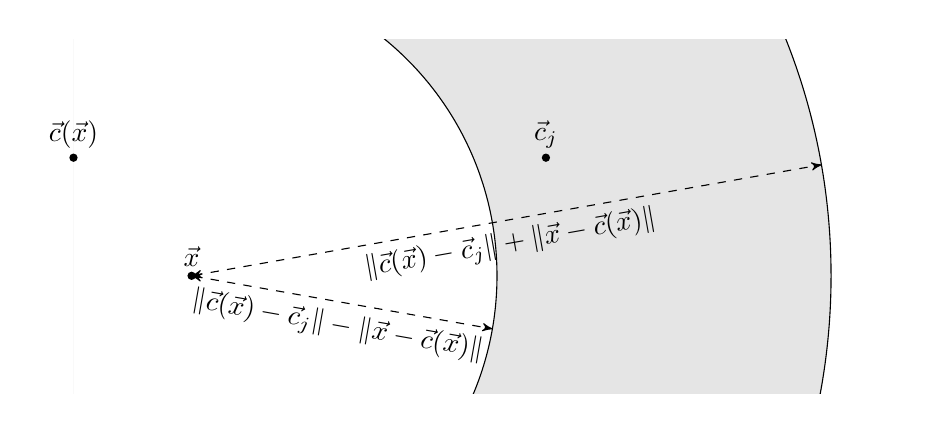
\begin{tikzpicture}[->,>=stealth',x=1.5cm, y=1.5cm, scale=1.0, transform shape,background rectangle/.style={fill=white}, show background rectangle]
\tikzset{dot/.style={circle,fill=#1,inner sep=0,minimum size=3pt}}

% centroids - that one that is moving
\coordinate (x) at (0,0);
\coordinate (cx) at (-1,1);
\coordinate (cj) at (3,1);

\begin{scope}[]
\clip (-1,2) rectangle (6,-1);
\draw[fill=black!10!white] (x) circle (5.4142);
\draw[fill=white] (x) circle (2.5858);
\end{scope}

\node[dot=black] at (x) {};
\node at (x) [above] {$\vec{x}$};
\node[dot=black] at (cx) {};
\node at (cx) [above] {$\vec{c}(\vec{x})$};
\node[dot=black] at (cj) {};
\node at (cj) [above] {$\vec{c}_j$};

\begin{scope}[rotate around={-10:(x)}]
\draw[dashed,<->] (x) -- +(2.5858,0);
\node at ($(x)+(1.2929,0)$) [below] {$\|\vec{c}(\vec{x})-\vec{c}_j\|-\|\vec{x}-\vec{c}(\vec{x})\|$};
\end{scope}

\begin{scope}[rotate around={10:(x)}]
\draw[dashed,<->] (x) -- +(5.4142,0);
\node at ($(x)+(2.7071,0)$) [below] {$\|\vec{c}(\vec{x})-\vec{c}_j\|+\|\vec{x}-\vec{c}(\vec{x})\|$};
\end{scope}

\end{tikzpicture}
\end{frame}

\begin{frame}{When triangle inequality helps 2/2}
  \usetikzlibrary{calc}
\usetikzlibrary{arrows}
\usetikzlibrary{decorations.pathreplacing}
\usetikzlibrary{backgrounds}

\newcommand{\samples}{100}

\providecommand{\x}{\vec{x}}
\providecommand{\cj}{\vec{c}_j}
\newcommand{\dstxxx}{4.1231}

\begin{tikzpicture}[->,>=stealth',x=1.5cm, y=1.5cm, scale=1.0, transform shape,background rectangle/.style={fill=white}, show background rectangle]
\tikzset{dot/.style={circle,fill=#1,inner sep=0,minimum size=3pt}}

% centroids - that one that is moving
\coordinate (x) at (0,0);
\coordinate (cj) at (4,1);
\coordinate (move) at (0,-2);

\begin{scope}[]
\clip (0,1.5) rectangle (6.5,-1.5);
\draw[fill=black!10!white] (x) circle (\dstxxx+2);
\draw[fill=white] (x) circle (\dstxxx-2);
\end{scope}

\node[dot=black] at (x) {};
\node at (x) [above] {$\vec{x}$};
\node[dot=black] at (cj) {};
\node at (cj) [above] {$\vec{c}_j$};

\node[dot=black,rotate around={-20:(cj)}] at ($(cj)+(move)$) {};
\node[,rotate around={-20:(cj)},rotate=20] at ($(cj)+(move)$) [below] {$\cj'$};

\begin{scope}[rotate around={-10:(x)}]
\draw[dashed,<->] (x) -- +(\dstxxx-2,0);
\node at ($(x)+(\dstxxx/2-1,0)$) [below] {$\|\x-\cj\|-\|\cj-\cj'\|$};
\end{scope}

\begin{scope}[rotate around={10:(x)}]
\draw[dashed,<->] (x) -- +(\dstxxx+2,0);
\node at ($(x)+(\dstxxx/2+1,0)$) [below] {$\|\x-\cj\|+\|\cj-\cj'\|$};
\end{scope}

\end{tikzpicture}
\end{frame}

\begin{frame}{Elkan's algorithm}
  \begin{itemize}
    \item One \emph{upper bound} $\ux$ on the distance to the closest centroid.
    \item $k$ \emph{lower bounds} $\lxcj$ on the distances between the
      point $\x$ and each centroid.
  \end{itemize}
  \begin{center}
    \usetikzlibrary{calc}
\usetikzlibrary{arrows}
\usetikzlibrary{decorations.pathreplacing}
\usetikzlibrary{backgrounds}

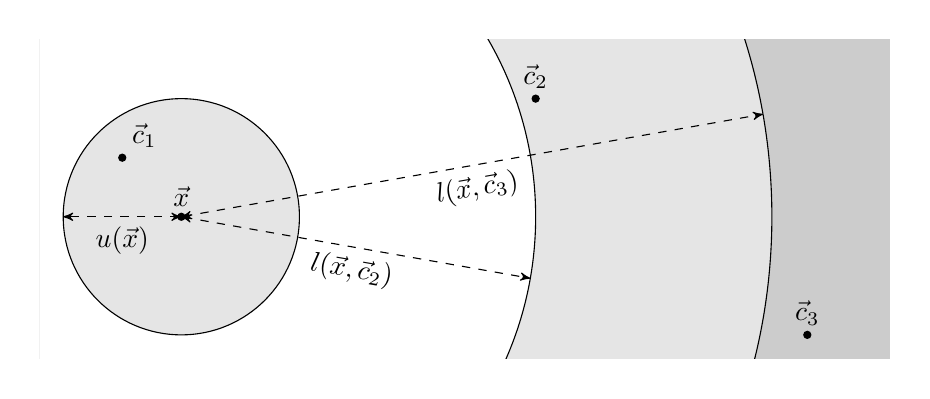
\begin{tikzpicture}[->,>=stealth',x=1.5cm, y=1.5cm, scale=1.0, transform shape,background rectangle/.style={fill=white}, show background rectangle]
\tikzset{dot/.style={circle,fill=#1,inner sep=0,minimum size=3pt}}

% centroids - that one that is moving
\coordinate (x) at (0,0);
\coordinate (c1) at (-0.5,0.5);
\coordinate (c2) at (3,1);
\coordinate (c3) at (5.3,-1);

\coordinate (cx) at (-0.5,0.5);
\coordinate (cj) at (3.3,1);

\begin{scope}[]
\clip (-1.2,1.5) rectangle (6,-1.2);

\draw[fill=black!20!white] (x) circle (10);
\draw[fill=black!10!white] (x) circle (5);
\draw[fill=white] (x) circle (3);

\draw[fill=black!10!white] (x) circle (1);

%\draw[fill=black!10!white] (x) circle (5.4142);
%\draw[fill=white] (x) circle (2.5858);
\end{scope}

\node[dot=black] at (x) {};
\node at (x) [above] {$\vec{x}$};
\node[dot=black] at (cx) {};
\node at (c1) [above right] {$\vec{c}_1$};
\node[dot=black] at (c2) {};
\node at (c2) [above] {$\vec{c}_2$};
\node[dot=black] at (c3) {};
\node at (c3) [above] {$\vec{c}_3$};

\draw[dashed,<->] (x) -- +(-1,0);
\node at (-0.5,0) [below] {$u(\vec{x})$};

\begin{scope}[rotate around={-10:(x)}]
\draw[dashed,<->] (x) -- +(3,0);
\node at ($(x)+(1.5,0)$) [below] {$l(\vec{x},\vec{c}_2)$};
\end{scope}

\begin{scope}[rotate around={10:(x)}]
\draw[dashed,<->] (x) -- +(5,0);
\node at ($(x)+(2.51,0)$) [below] {$l(\vec{x},\vec{c}_3)$};
\end{scope}

\end{tikzpicture}
  \end{center}
\end{frame}

\begin{frame}{Hamerly's algorithm}
  \begin{itemize}
    \item One \emph{upper bound} $u(\vec{x})$.
    \item One \emph{lower bound} $l(\vec{x})$ that stands for a lower bound on the distance
      between the point $\vec{x}$ and its second closest centroid.
  \end{itemize}
  \begin{center}
    \usetikzlibrary{calc}
\usetikzlibrary{arrows}
\usetikzlibrary{decorations.pathreplacing}
\usetikzlibrary{backgrounds}

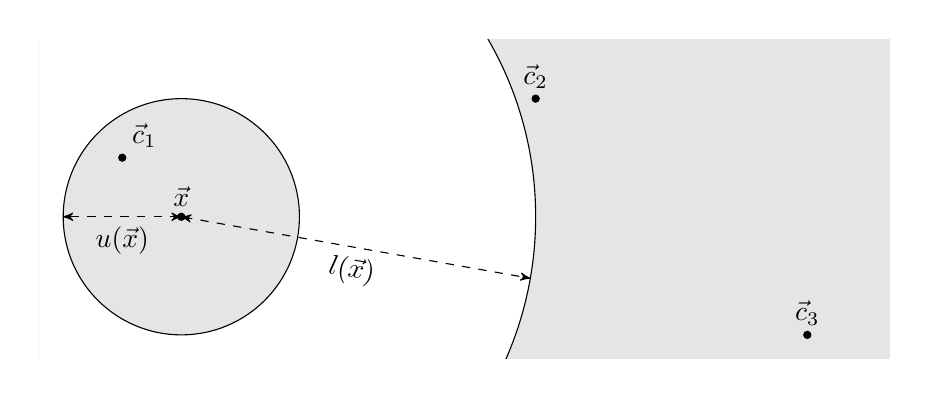
\begin{tikzpicture}[->,>=stealth',x=1.5cm, y=1.5cm, scale=1.0, transform shape,background rectangle/.style={fill=white}, show background rectangle]
\tikzset{dot/.style={circle,fill=#1,inner sep=0,minimum size=3pt}}

% centroids - that one that is moving
\coordinate (x) at (0,0);
\coordinate (c1) at (-0.5,0.5);
\coordinate (c2) at (3,1);
\coordinate (c3) at (5.3,-1);

\coordinate (cx) at (-0.5,0.5);
\coordinate (cj) at (3.3,1);

\begin{scope}[]
\clip (-1.2,1.5) rectangle (6,-1.2);

%\draw[fill=black!20!white] (x) circle (10);
\draw[fill=black!10!white] (x) circle (10);
\draw[fill=white] (x) circle (3);

\draw[fill=black!10!white] (x) circle (1);

%\draw[fill=black!10!white] (x) circle (5.4142);
%\draw[fill=white] (x) circle (2.5858);
\end{scope}

\node[dot=black] at (x) {};
\node at (x) [above] {$\vec{x}$};
\node[dot=black] at (cx) {};
\node at (c1) [above right] {$\vec{c}_1$};
\node[dot=black] at (c2) {};
\node at (c2) [above] {$\vec{c}_2$};
\node[dot=black] at (c3) {};
\node at (c3) [above] {$\vec{c}_3$};

\draw[dashed,<->] (x) -- +(-1,0);
\node at (-0.5,0) [below] {$u(\vec{x})$};

\begin{scope}[rotate around={-10:(x)}]
\draw[dashed,<->] (x) -- +(3,0);
\node at ($(x)+(1.5,0)$) [below] {$l(\vec{x})$};
\end{scope}

\end{tikzpicture}
  \end{center}
\end{frame}

\begin{frame}{Heap algorithm}
  \begin{itemize}
    \item The upper bound and the lower bound are combined into a single bound $$\lux = \lx - \ux.$$
    \item Points are put into $k$ heaps, one for each cluster.
    \item Once a point has $\lux > 0$, all remaining points can be skipped.
    \item All points in the cluster have the same lower/upper bound update.
    \item Bounds stored relative to the center movement (no need to update key in each iteration).
  \end{itemize}
\end{frame}

\begin{frame}{Annular algorithm}
  \begin{itemize}
    \item Modification of Hamerly's algorithm.
    \item Searches only centroids lying in an annulus centered at origin.
  \end{itemize}
  \begin{center}
    \includegraphics[scale=1.2, page=32, trim=8.7cm 2.5cm 0.8cm 3.8cm, clip]{files/fast_kmeans_talk_20140515.pdf}
    \newline
    [Image taken from \url{http://cs.ecs.baylor.edu/~hamerly/software/fast\_kmeans\_talk\_20140515.pdf}, pg.32]  
  \end{center}
\end{frame}

\plain{Proposed changes}

\section{Tighter update}

\begin{frame}{Motivation}
  \begin{itemize}
    \item We assume the worst case while we update the upper/lower bounds.
    \item Points in cluster are not everywhere in space.
    \item Points in cluster fulfill some locality.
    \item When a centroid move away, the lower bound does not have to shrink.
  \end{itemize}
\end{frame}

\begin{frame}{How to describe the locality of a cluster?}
  \begin{itemize}
    \item We use the upper bound.
    \item Any point is in distance $\ux$ from its closest centroid.
    \item Therefore each point is at most
      \begin{equation*}
         \mci = \max_{\vec{y} \mid \vec{c}(\vec{y}) = \ci} u(\vec{y}).
      \end{equation*}
      from its closest centroid $\ci$.
  \end{itemize}
\end{frame}

\begin{frame}{How much we can update the lower bound?}
  \begin{itemize}
     \item The update $\deltaxcj$ of $\lxcj$ must fulfill
       \begin{equation*}
         \deltaxcj \geq \distxcj - \distxcjp
       \end{equation*}
     \item The update is at least the difference between the old and new distance.
     \item Denote $\distxcj - \distxcjp = f(\x)$.
  \end{itemize}
\end{frame}

\begin{frame}{What is $f(\x) = \distxcj - \distxcjp$}
  \begin{itemize}
    \item Fix $f(\x) = z$.
    \item It is a hyperbola with focal points $\cj$ and $\cj'$.
  \end{itemize}
  \begin{center}
    \usetikzlibrary{calc}
\usetikzlibrary{arrows}
\usetikzlibrary{decorations.pathreplacing}

\newcommand{\samples}{100}

\providecommand{\x}{\vec{x}}
\providecommand{\cj}{\vec{c}_j}
\providecommand{\ci}{\vec{c}_i}


\begin{tikzpicture}[x=1in, y=1in, scale=0.7, transform shape]

% centroids - that one that is moving
\coordinate (c) at (0,1);
\coordinate (c') at (0,-1);
\tikzset{dot/.style={circle,fill=#1,inner sep=0,minimum size=3pt}}
\node[dot=black] at (c) {};
\node at (c) [above right] {$\cj$};
\node[dot=black] at (c') {};
\node at (c') [below right] {$\cj'$};

% draw the hyperbola
\begin{scope}[]
\clip (-1,-1.25) rectangle (1,1.25);
\draw[] plot[variable=\t,samples=\samples,domain=-64:64] ({0.7071*tan(\t)},{-0.7071*sec(\t)});
\end{scope}

% draw axis
%\draw (-1,0) -- (2,0);
%\draw (0,-1.2) -- (0,1.2);

% draw the asymptote
%\draw[dashed] (0,0) -- (1.2,-1.2);
% draw the s vector
%\coordinate (s) at (0.9,-0.9);
%\draw[thick,->] (0,0) -> (s);
%\node[dot=black] at (s) {};
%\node at (s) [above=5pt] {$\vec{s}$};

% the center ci
%\coordinate (ci) at (0.5,0.5);
%\node[dot=black] at ($(s)+(ci)$) {};
%\node at ($(s)+(ci)$) [below right] {$\ci$};
% the circle
%\draw ($(s)+(ci)$) circle (0.7071);

% the radius
%\draw[color=gray, dashed] ($(s)+(ci)$) -- (s);
%\node[color=gray] at ($(s)+0.5*(ci)$) [above left] {$r$};

% axis of hyperbola
%\draw[color=gray,decorate, decoration={brace, amplitude=4pt}] (0,-0.7071) -- (0,0);
%\node at ($0.35*(c')$) [left = 4pt] {$a$};
%\draw[color=gray, dashed] ($0.5*(c')$) -- +(0.5,0);
%\node[color=gray] at ($0.5*(c')+(0.25,0)$) [above] {$b$};

% point x
%\coordinate (x) at (1,-0.1);
%\node[dot=gray] at (x) {};
%\node[color=gray] at (x) [below] {$\x$};

\end{tikzpicture}
  \end{center}
\end{frame}

\begin{frame}{Where we can use update $\deltaxcj = z$}
  \begin{center}
    \usetikzlibrary{calc}
\usetikzlibrary{arrows}
\usetikzlibrary{decorations.pathreplacing}

\newcommand{\samples}{100}

\providecommand{\x}{\vec{x}}
\providecommand{\cj}{\vec{c}_j}
\providecommand{\ci}{\vec{c}_i}


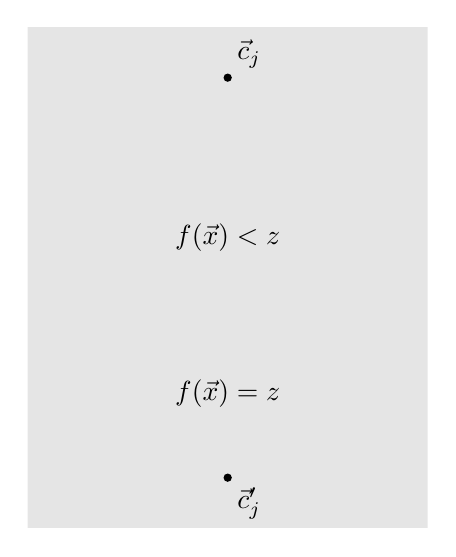
\begin{tikzpicture}[x=1in, y=1in, scale=1.0, transform shape]

% draw the hyperbola
\begin{scope}[]
\clip (-1,-1.25) rectangle (1,1.25);
\draw[fill=black!10!white] plot[variable=\t,samples=\samples,domain=-64:64] ({0.7071*tan(\t)},{-0.7071*sec(\t)}) -- (2,2) -- (-2,2);
\end{scope}

\node at (0,-0.7) [above] {$f(\x) = z$};

% centroids - that one that is moving
\coordinate (c) at (0,1);
\coordinate (c') at (0,-1);
\tikzset{dot/.style={circle,fill=#1,inner sep=0,minimum size=3pt}}
\node[dot=black] at (c) {};
\node at (c) [above right] {$\cj$};
\node[dot=black] at (c') {};
\node at (c') [below right] {$\cj'$};

\node at (0,0.2) {$f(\vec{x}) < z$};

% draw axis
%\draw (-1,0) -- (2,0);
%\draw (0,-1.2) -- (0,1.2);

% draw the asymptote
%\draw[dashed] (0,0) -- (1.2,-1.2);
% draw the s vector
%\coordinate (s) at (0.9,-0.9);
%\draw[thick,->] (0,0) -> (s);
%\node[dot=black] at (s) {};
%\node at (s) [above=5pt] {$\vec{s}$};

% the center ci
%\coordinate (ci) at (0.5,0.5);
%\node[dot=black] at ($(s)+(ci)$) {};
%\node at ($(s)+(ci)$) [below right] {$\ci$};
% the circle
%\draw ($(s)+(ci)$) circle (0.7071);

% the radius
%\draw[color=gray, dashed] ($(s)+(ci)$) -- (s);
%\node[color=gray] at ($(s)+0.5*(ci)$) [above left] {$r$};

% axis of hyperbola
%\draw[color=gray,decorate, decoration={brace, amplitude=4pt}] (0,-0.7071) -- (0,0);
%\node at ($0.35*(c')$) [left = 4pt] {$a$};
%\draw[color=gray, dashed] ($0.5*(c')$) -- +(0.5,0);
%\node[color=gray] at ($0.5*(c')+(0.25,0)$) [above] {$b$};

% point x
%\coordinate (x) at (1,-0.1);
%\node[dot=gray] at (x) {};
%\node[color=gray] at (x) [below] {$\x$};

\end{tikzpicture}
  \end{center}
\end{frame}

\begin{frame}{There is somewhere point $\x$ ...}
  \begin{center}
    \usetikzlibrary{calc}
\usetikzlibrary{arrows}
\usetikzlibrary{decorations.pathreplacing}

\newcommand{\samples}{100}

\providecommand{\x}{\vec{x}}
\providecommand{\cj}{\vec{c}_j}
\providecommand{\ci}{\vec{c}_i}


\begin{tikzpicture}[x=1in, y=1in, scale=1.0, transform shape]

% centroids - that one that is moving
\coordinate (c) at (0,1);
\coordinate (c') at (0,-1);
\tikzset{dot/.style={circle,fill=#1,inner sep=0,minimum size=3pt}}
\node[dot=black] at (c) {};
\node at (c) [above right] {$\cj$};
\node[dot=black] at (c') {};
\node at (c') [below right] {$\cj'$};

% draw the hyperbola
\begin{scope}[]
\clip (-1,-1.25) rectangle (1,1.25);
\draw[] plot[variable=\t,samples=\samples,domain=-64:64] ({0.7071*tan(\t)},{-0.7071*sec(\t)});
\end{scope}

% draw axis
%\draw (-1,0) -- (2,0);
%\draw (0,-1.2) -- (0,1.2);

% draw the asymptote
%\draw[dashed] (0,0) -- (1.2,-1.2);
% draw the s vector
%\coordinate (s) at (0.9,-0.9);
%\draw[thick,->] (0,0) -> (s);
%\node[dot=black] at (s) {};
%\node at (s) [above=5pt] {$\vec{s}$};

% the center ci
%\coordinate (ci) at (0.5,0.5);
%\node[dot=black] at ($(s)+(ci)$) {};
%\node at ($(s)+(ci)$) [below right] {$\ci$};
% the circle
%\draw ($(s)+(ci)$) circle (0.7071);

% the radius
%\draw[color=gray, dashed] ($(s)+(ci)$) -- (s);
%\node[color=gray] at ($(s)+0.5*(ci)$) [above left] {$r$};

% axis of hyperbola
%\draw[color=gray,decorate, decoration={brace, amplitude=4pt}] (0,-0.7071) -- (0,0);
%\node at ($0.35*(c')$) [left = 4pt] {$a$};
%\draw[color=gray, dashed] ($0.5*(c')$) -- +(0.5,0);
%\node[color=gray] at ($0.5*(c')+(0.25,0)$) [above] {$b$};

% point x
\coordinate (x) at (1,-0.1);
\node[dot=black] at (x) {};
\node[color=black] at (x) [below] {$\x$};

\end{tikzpicture}
  \end{center}
\end{frame}

\begin{frame}{\ldots actually somewhere in the cluster}
  \begin{center}
    \usetikzlibrary{calc}
\usetikzlibrary{arrows}
\usetikzlibrary{decorations.pathreplacing}

\newcommand{\samples}{100}

\providecommand{\x}{\vec{x}}
\providecommand{\cj}{\vec{c}_j}
\providecommand{\ci}{\vec{c}_i}


\begin{tikzpicture}[x=1in, y=1in, scale=1.0, transform shape]

% centroids - that one that is moving
\coordinate (c) at (0,1);
\coordinate (c') at (0,-1);
\tikzset{dot/.style={circle,fill=#1,inner sep=0,minimum size=3pt}}
\node[dot=black] at (c) {};
\node at (c) [above right] {$\cj$};
\node[dot=black] at (c') {};
\node at (c') [below right] {$\cj'$};

% draw the hyperbola
\begin{scope}[]
\clip (-1,-1.25) rectangle (1,1.25);
\draw[] plot[variable=\t,samples=\samples,domain=-64:64] ({0.7071*tan(\t)},{-0.7071*sec(\t)});
\end{scope}

% draw axis
%\draw (-1,0) -- (2,0);
%\draw (0,-1.2) -- (0,1.2);

% draw the asymptote
%\draw[dashed] (0,0) -- (1.2,-1.2);
% draw the s vector
\coordinate (s) at (0.9,-0.9);
%\draw[thick,->] (0,0) -> (s);
%\node[dot=black] at (s) {};
%\node at (s) [above=5pt] {$\vec{s}$};

% the center ci
\coordinate (ci) at (0.5,0.5);
\node[dot=black] at ($(s)+(ci)$) {};
\node at ($(s)+(ci)$) [below right] {$\ci$};
% the circle
\draw ($(s)+(ci)$) circle (0.7071);

% the radius
\draw[color=gray, dashed] ($(s)+(ci)$) -- (s);
\node[color=gray] at ($(s)+0.5*(ci)$) [above left] {$r$};

% axis of hyperbola
%\draw[color=gray,decorate, decoration={brace, amplitude=4pt}] (0,-0.7071) -- (0,0);
%\node at ($0.35*(c')$) [left = 4pt] {$a$};
%\draw[color=gray, dashed] ($0.5*(c')$) -- +(0.5,0);
%\node[color=gray] at ($0.5*(c')+(0.25,0)$) [above] {$b$};

% point x
\coordinate (x) at (1,-0.1);
\node[dot=gray] at (x) {};
\node[color=gray] at (x) [below] {$\x$};

\end{tikzpicture}
  \end{center}
\end{frame}

\begin{frame}{Find the asymptote}
  \begin{center}
    \usetikzlibrary{calc}
\usetikzlibrary{arrows}
\usetikzlibrary{decorations.pathreplacing}

\newcommand{\samples}{100}

\providecommand{\x}{\vec{x}}
\providecommand{\cj}{\vec{c}_j}
\providecommand{\ci}{\vec{c}_i}


\begin{tikzpicture}[x=1in, y=1in, scale=1.0, transform shape]

% centroids - that one that is moving
\coordinate (c) at (0,1);
\coordinate (c') at (0,-1);
\tikzset{dot/.style={circle,fill=#1,inner sep=0,minimum size=3pt}}
\node[dot=black] at (c) {};
\node at (c) [above right] {$\cj$};
\node[dot=black] at (c') {};
\node at (c') [below right] {$\cj'$};

% draw the hyperbola
\begin{scope}[]
\clip (-1,-1.25) rectangle (1,1.25);
\draw[] plot[variable=\t,samples=\samples,domain=-64:64] ({0.7071*tan(\t)},{-0.7071*sec(\t)});
\end{scope}

% draw axis
\draw (-1,0) -- (2,0);
\draw (0,-1.2) -- (0,1.2);

% draw the asymptote
\draw[dashed] (0,0) -- (1.2,-1.2);
% draw the s vector
\coordinate (s) at (0.9,-0.9);
%\draw[thick,->] (0,0) -> (s);
%\node[dot=black] at (s) {};
%\node at (s) [above=5pt] {$\vec{s}$};

% the center ci
\coordinate (ci) at (0.5,0.5);
\node[dot=black] at ($(s)+(ci)$) {};
\node at ($(s)+(ci)$) [below right] {$\ci$};
% the circle
\draw ($(s)+(ci)$) circle (0.7071);

% the radius
\draw[color=gray, dashed] ($(s)+(ci)$) -- (s);
\node[color=gray] at ($(s)+0.5*(ci)$) [above left] {$r$};

% axis of hyperbola
%\draw[color=gray,decorate, decoration={brace, amplitude=4pt}] (0,-0.7071) -- (0,0);
%\node at ($0.35*(c')$) [left = 4pt] {$a$};
%\draw[color=gray, dashed] ($0.5*(c')$) -- +(0.5,0);
%\node[color=gray] at ($0.5*(c')+(0.25,0)$) [above] {$b$};

% point x
\coordinate (x) at (1,-0.1);
\node[dot=gray] at (x) {};
\node[color=gray] at (x) [below] {$\x$};

\end{tikzpicture}
  \end{center}
\end{frame}

\begin{frame}{\ldots and the point where it touches the circle}
  \begin{center}
    \usetikzlibrary{calc}
\usetikzlibrary{arrows}
\usetikzlibrary{decorations.pathreplacing}

\newcommand{\samples}{100}

\providecommand{\x}{\vec{x}}
\providecommand{\cj}{\vec{c}_j}
\providecommand{\ci}{\vec{c}_i}


\begin{tikzpicture}[x=1in, y=1in, scale=1.0, transform shape]

% centroids - that one that is moving
\coordinate (c) at (0,1);
\coordinate (c') at (0,-1);
\tikzset{dot/.style={circle,fill=#1,inner sep=0,minimum size=3pt}}
\node[dot=black] at (c) {};
\node at (c) [above right] {$\cj$};
\node[dot=black] at (c') {};
\node at (c') [below right] {$\cj'$};

% draw the hyperbola
\begin{scope}[]
\clip (-1,-1.25) rectangle (1,1.25);
\draw[] plot[variable=\t,samples=\samples,domain=-64:64] ({0.7071*tan(\t)},{-0.7071*sec(\t)});
\end{scope}

% draw axis
\draw (-1,0) -- (2,0);
\draw (0,-1.2) -- (0,1.2);

% draw the asymptote
\draw[dashed] (0,0) -- (1.2,-1.2);
% draw the s vector
\coordinate (s) at (0.9,-0.9);
\draw[thick,->] (0,0) -> (s);
\node[dot=black] at (s) {};
\node at (s) [above=5pt] {$\vec{s}$};

% the center ci
\coordinate (ci) at (0.5,0.5);
\node[dot=black] at ($(s)+(ci)$) {};
\node at ($(s)+(ci)$) [below right] {$\ci$};
% the circle
\draw ($(s)+(ci)$) circle (0.7071);

% the radius
\draw[color=gray, dashed] ($(s)+(ci)$) -- (s);
\node[color=gray] at ($(s)+0.5*(ci)$) [above left] {$r$};

% axis of hyperbola
%\draw[color=gray,decorate, decoration={brace, amplitude=4pt}] (0,-0.7071) -- (0,0);
%\node at ($0.35*(c')$) [left = 4pt] {$a$};
%\draw[color=gray, dashed] ($0.5*(c')$) -- +(0.5,0);
%\node[color=gray] at ($0.5*(c')+(0.25,0)$) [above] {$b$};

% point x
\coordinate (x) at (1,-0.1);
\node[dot=gray] at (x) {};
\node[color=gray] at (x) [below] {$\x$};

\end{tikzpicture}
  \end{center}
\end{frame}

\begin{frame}{Update calculation}
\vspace{-0.5cm}
\begin{lemma}
Suppose that $\x \in \R^2$, $\ux \leq r \in \Rpz$ and $\ci = (c_{ix}, c_{iy})$,
where $c_{ix} > r$ and $c_{iy} \leq r$. Let $\cj=(0,1)$ and $\cj'=(0,-1)$. Then
\begin{equation*}
    \deltaxcj =
        2\frac{
            c_{ix} r
            -
            c_{iy} \sqrt{\| \ci \|^2 - r^2}
        }{
             \| \ci \|^2
        }
\end{equation*}
is a valid update of the lower bound $\lxcj$.
\end{lemma}
  \begin{center}
    \usetikzlibrary{calc}
\usetikzlibrary{arrows}
\usetikzlibrary{decorations.pathreplacing}

\newcommand{\samples}{100}

\providecommand{\x}{\vec{x}}
\providecommand{\cj}{\vec{c}_j}
\providecommand{\ci}{\vec{c}_i}


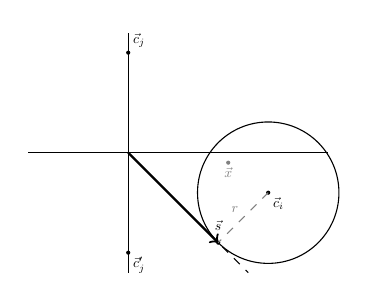
\begin{tikzpicture}[x=1in, y=1in, scale=0.5, transform shape]

% centroids - that one that is moving
\coordinate (c) at (0,1);
\coordinate (c') at (0,-1);
\tikzset{dot/.style={circle,fill=#1,inner sep=0,minimum size=3pt}}
\node[dot=black] at (c) {};
\node at (c) [above right] {$\cj$};
\node[dot=black] at (c') {};
\node at (c') [below right] {$\cj'$};

% draw the hyperbola
\begin{scope}[]
\clip (-1,-1.25) rectangle (1,1.25);
\draw[] plot[variable=\t,samples=\samples,domain=-64:64] ({0.7071*tan(\t)},{-0.7071*sec(\t)});
\end{scope}

% draw axis
\draw (-1,0) -- (2,0);
\draw (0,-1.2) -- (0,1.2);

% draw the asymptote
\draw[dashed] (0,0) -- (1.2,-1.2);
% draw the s vector
\coordinate (s) at (0.9,-0.9);
\draw[thick,->] (0,0) -> (s);
\node[dot=black] at (s) {};
\node at (s) [above=5pt] {$\vec{s}$};

% the center ci
\coordinate (ci) at (0.5,0.5);
\node[dot=black] at ($(s)+(ci)$) {};
\node at ($(s)+(ci)$) [below right] {$\ci$};
% the circle
\draw ($(s)+(ci)$) circle (0.7071);

% the radius
\draw[color=gray, dashed] ($(s)+(ci)$) -- (s);
\node[color=gray] at ($(s)+0.5*(ci)$) [above left] {$r$};

% axis of hyperbola
%\draw[color=gray,decorate, decoration={brace, amplitude=4pt}] (0,-0.7071) -- (0,0);
%\node at ($0.35*(c')$) [left = 4pt] {$a$};
%\draw[color=gray, dashed] ($0.5*(c')$) -- +(0.5,0);
%\node[color=gray] at ($0.5*(c')+(0.25,0)$) [above] {$b$};

% point x
\coordinate (x) at (1,-0.1);
\node[dot=gray] at (x) {};
\node[color=gray] at (x) [below] {$\x$};

\end{tikzpicture}
  \end{center}
\end{frame}

\begin{frame}{Multidimensional case}
  \begin{center}
    \usetikzlibrary{calc}
\usetikzlibrary{arrows}
\usetikzlibrary{decorations.pathreplacing}

\newcommand{\samples}{100}

\providecommand{\x}{\vec{x}}
\providecommand{\cj}{\vec{c}_j}
\providecommand{\ci}{\vec{c}_i}


\begin{tikzpicture}[x=1in, y=1in, scale=1.0, transform shape]

% centroids - that one that is moving
\coordinate (c) at (0,1);
\coordinate (c') at (0,-1);
\tikzset{dot/.style={circle,fill=#1,inner sep=0,minimum size=3pt}}
\node[dot=black] at (c) {};
\node at (c) [above right] {$\cj$};
\node[dot=black] at (c') {};
\node at (c') [below right] {$\cj'$};

% draw the hyperbola
\begin{scope}[]
\clip (-1,-1.25) rectangle (1,1.25);
\draw[] plot[variable=\t,samples=\samples,domain=-64:64] ({0.7071*tan(\t)},{-0.7071*sec(\t)});
\end{scope}

% draw axis
\draw (-1,0) -- (2,0);
\draw (0,-1.2) -- (0,1.2);

% draw the asymptote
\draw[dashed] (0,0) -- (1.2,-1.2);
% draw the s vector
\coordinate (s) at (0.9,-0.9);
\draw[thick,->] (0,0) -> (s);
\node[dot=black] at (s) {};
\node at (s) [above=5pt] {$\vec{s}$};

% the center ci
\coordinate (ci) at (0.5,0.5);
\node[dot=black] at ($(s)+(ci)$) {};
\node at ($(s)+(ci)$) [below right] {$\ci$};
% the circle
\draw ($(s)+(ci)$) circle (0.7071);

% the radius
\draw[color=gray, dashed] ($(s)+(ci)$) -- (s);
\node[color=gray] at ($(s)+0.5*(ci)$) [above left] {$r$};

% axis of hyperbola
%\draw[color=gray,decorate, decoration={brace, amplitude=4pt}] (0,-0.7071) -- (0,0);
%\node at ($0.35*(c')$) [left = 4pt] {$a$};
%\draw[color=gray, dashed] ($0.5*(c')$) -- +(0.5,0);
%\node[color=gray] at ($0.5*(c')+(0.25,0)$) [above] {$b$};

% point x
\coordinate (x) at (1,-0.1);
\node[dot=gray] at (x) {};
\node[color=gray] at (x) [below] {$\x$};

\end{tikzpicture}
  \end{center}
\end{frame}

\begin{frame}{Projection}
  \begin{align*}
    \mathsf{c}_{ix} &= 2 \frac{\| \vec{P}(\ci) - \ci \| }{ \movcj },
    \\
    \mathsf{c}_{iy} &= 1-2t,
    \\
    r &= 2 \frac{\mci}{\movcj},
  \end{align*}
  where
  \begin{equation*}
    \vec{P}(\ci) = \cj + t \cdot (\cj' - \cj)= \cj + \frac{(\ci-\cj)^T(\cj' - \cj)}{\movcj^2} (\cj' - \cj)
  \end{equation*}
  is the projection of $\ci$ onto line through $\cj$ and $\cj'$.
\end{frame}

\begin{frame}{Application to various algorithms}
  \begin{itemize}
    \item Applicable directly to Elkan's algorithm.
    \item Hamerly's and annular algorithm?
    \item Heap algorithm?
  \end{itemize}
\end{frame}

\section{Cluster neighbors}

\begin{frame}{Neighbor}
  \begin{itemize}
    \item In Hamerly's algorithm we need to know the distance to the second closest neighbor in the innermost loop.
    \item What if we knew what was the second closest centroid?
  \end{itemize}
  \begin{definition}
    The \emph{neighbor} of a centroid $\ci$ is any centroid $\cj$
    that is closest or second closest to any point assigned to $\ci$.
  \end{definition}
\end{frame}

\begin{frame}{How to find out which centroids are neighbors}
  \begin{theorem}
    Any neighbor $\cj$ of a centroid $\ci$ must fulfill the condition
    \begin{equation}
      m(\ci) + s(\ci) \geq \frac{1}{2} \| \ci - \cj \|.
    \end{equation}
  \end{theorem}
  $\sci$ is the distance from $\ci$ to closest other centroid, i.e.
  \begin{equation}
    \sci = \frac{1}{2} \min_{j \in \{1,2, \ldots, i-1, i+1, \ldots, k\}} \| \cj - \ci \|.
  \end{equation}
\end{frame}

\begin{frame}{Why?}
  \begin{itemize}
    \item If the condition is violated, we know that for $\x$ assigned to $\ci$:
    \begin{itemize}
      \item $\ci$ is closer to $\x$ than $\cj$ and
      \item the closest other centroid to $\ci$ is closer to $\x$ than $\cj$.
    \end{itemize}
  \end{itemize}
\end{frame}

\section{Explicit upper bound for heap algorithm}

\begin{frame}{Problems of heap algorithm}
  \begin{itemize}
    \item The heap algorithm cannot tighten the upper bound (left as open problem).
    \item How do we evaluate the maximal upper bound $\mci$?
  \end{itemize}
\end{frame}

\begin{frame}{Solution}
  \begin{itemize}
    \item[\no] Store the $\ux$ together with $\lux$
    \begin{itemize}
      \item Breaks the asymptotic complexity.
    \end{itemize}
    \item[\yes] Store the $\ux$ relative to the center movement.
    \begin{itemize}
      \item Follows the virtue of the heap algorithm.
      \item To get the $\mci$ we need to put points in the heaps.
    \end{itemize}
  \end{itemize}
\end{frame}

\section{Other changes}

\begin{frame}{Other changes}
  \begin{enumerate}
    \item Tweaking the first iteration
    \item Storing the bounds relative to the sum of updates for Elkan's algorithm
    \item Using stronger condition for neighbors in Elkan's algorithm
  \end{enumerate}
\end{frame}

\section{Experimental results}

\begin{frame}{Experimental results}
  \begin{itemize}
    \item Same conditions, same initialization.
    \item Runtime averaged over $10$ repeats.
    \item Sources: \url{https://github.com/petrrysavy/baylorml} (based on code by G. Hamerly and J. Drake)
  \end{itemize}
\end{frame}

\begin{frame}{Datasets}
  \small
\centering
\label{tab:datasets}
\begin{tabularx}{\textwidth}{lXrrr}
\hline
Name & Description & Points $n$ & Dimension $d$ & $k$ \\
\hline
Uniform-$d$ & Synthetic data from uniform distribution & $1 \, 000 \, 000$ & 2/3/5/7/10/15 & 50 \\
Clustered-$d$ & Synthetic data, 50 clusters & $1 \, 000 \, 000$ & 2/3/5/7/10/15 & 50 \\
\href{http://cs.joensuu.fi/sipu/datasets/}{BIRCH} & Synthetic grid $10\times 10$ Gaussian clusters & $100 \, 000$ & $2$ & $100$ \\
\href{https://archive.ics.uci.edu/ml/datasets/Covertype}{Covertype} & Forest CoverType dataset & $581 \, 012$ & 54 & 8 \\
\href{http://yann.lecun.com/exdb/mnist/}{MNIST-784} & Handwritten digit images $28\times 28\,\mathrm{px}$ & $60 \, 000$ & $784$ & $10$ \\
MNIST-50 & Random linear projection of MNIST-784 & $60 \, 000$ & $50$ & $10$ \\
\hline
\end{tabularx}
\end{frame}

\begin{frame}{Algorithms}
  \vspace*{-1.1cm}
  \centering
  \small
  \begin{tabularx}{\textwidth}{lcccccX}
\hline
Algorithm & T. update & Neighbors & $\ux$ in heap & Elkan & 1st iteration  \\
\hline
Lloyd        &       &       &       &       &      \\
Compare      &       &       &       &       &      \\
Sort         &       &       &       &       &      \\
Elkan        &       &       &       &       &      \\
ElkanA       & \yes  &       &       &       &      \\
ElkanAB      & \yes  & \yes  &       &       &      \\
ElkanABD     & \yes  & \yes  &       & \yes  &      \\
Hamerly      &       &       &       &       &      \\
HamerlyA     & \yes  &       &       &       &      \\
HamerlyAB    & \yes  & \yes  &       &       &      \\
HamerlyABE   & \yes  & \yes  &       &       & \yes \\
HamerlyB     &       & \yes  &       &       &      \\
Heap         &       &       &       &       &      \\
HeapA        & \yes  &       &       &       &      \\
HeapAC       & \yes  &       & \yes  &       &      \\
HeapABC      & \yes  & \yes  & \yes  &       &      \\
Annulus      &       &       &       &       &      \\
AnnulusA     & \yes  &       &       &       &      \\
\hline
\end{tabularx}
\end{frame}

\begin{frame}{Runtime (Relative speedup to Lloyd's algorithm)}
\centering
\begin{tikzpicture}[scale=1]
\begin{axis}[ybar,
    symbolic x coords={
		Lloyd, Compare, Sort,
		Elkan, ElkanA, ElkanAB, ElkanABD,
		Hamerly, HamerlyA, HamerlyAB, HamerlyABE, HamerlyB,
		Heap, HeapA, HeapAC, HeapABC,
		Annulus, AnnulusA
	},
	xticklabels={Lloyd, \strongplot{Compare}, \strongplot{Sort},
		Elkan, ElkanA, ElkanAB, ElkanABD,
		\strongplot{Hamerly}, \strongplot{HamerlyA}, \strongplot{HamerlyAB}, \strongplot{HamerlyABE}, \strongplot{HamerlyB},
		Heap, HeapA, HeapAC, HeapABC,
		\strongplot{Annulus}, \strongplot{AnnulusA}},
	xtick=data,
    ymin=0,
    x tick label style={rotate=45,anchor=east},
    width=\plotwidth,
    height=\plotheight,
    bar width=1.5pt,
    ylabel={$\times$ faster than Lloyd's algorithm},
    legend pos=north west,
    ]
\addplot table [x={algo}, y expr={18.0945/\thisrow{birch}}] {\runtimestable};
\addplot table [x={algo}, y expr={19.9696/\thisrow{mnist50}}] {\runtimestable};
\addplot table [x={algo}, y expr={433.347/\thisrow{d5}}] {\runtimestable};
\addplot table [x={algo}, y expr={496.4453/\thisrow{u2}}] {\runtimestable};
\legend{BIRCH, MNIST-50, Clustered $d=5$, Uniform $d=2$}
\end{axis}
\end{tikzpicture}
\end{frame}

\begin{frame}{Number of distance calculations}
\centering
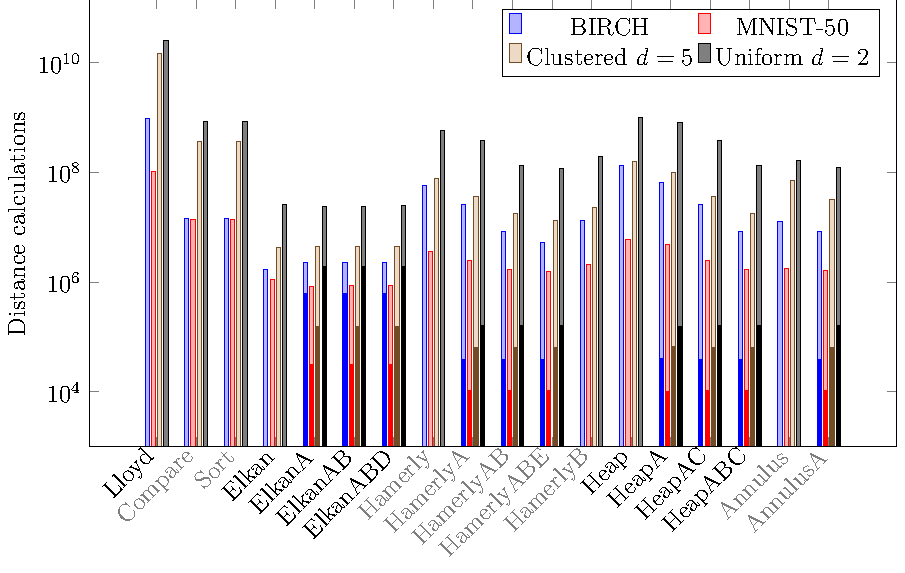
\includegraphics[width=\textwidth]{files/distplot.pdf}
\end{frame}

\begin{frame}{Average lower bound update per bound}
\begin{tikzpicture}[scale=1]
\begin{axis}[ybar,
    symbolic x coords={
		Elkan, ElkanA, ElkanAB, ElkanABD, Hamerly, HamerlyA, HamerlyAB, HamerlyABE, HamerlyB, Heap, HeapA, HeapAC, HeapABC, Annulus, AnnulusA
	},
	xtick=data,
	xticklabels={Elkan, ElkanA, ElkanAB, ElkanABD,
		\strongplot{Hamerly}, \strongplot{HamerlyA}, \strongplot{HamerlyAB}, \strongplot{HamerlyABE}, \strongplot{HamerlyB},
		Heap, HeapA, HeapAC, HeapABC,
		\strongplot{Annulus}, \strongplot{AnnulusA}},
    ymin=0,
    x tick label style={rotate=45,anchor=east},
    width=\plotwidth,
    height=\plotheight,
    bar width=1.5pt,
    ylabel={Average lower bound update},
    legend pos=north west,
    legend style={font=\scriptsize}
    ]
%\addplot table [x={eang}, y expr={\thisrowno{2}/\thisrow{1}/\thisrowno{3}/3933.9249}] {\updatestable};
\addplot table [x={eang}, y expr={\thisrow{birch}/\thisrow{bnd}/3.62994e10}] {\updatestable};
\addplot table [x={eang}, y expr={\thisrow{mnist50}/\thisrow{bounds}/1.06419e+09}] {\updatestable};
\addplot table [x={eang}, y expr={\thisrow{clusters5}/\thisrow{bounds}/1.15264e+06}] {\updatestable};
\addplot table [x={eang}, y expr={\thisrow{u2}/\thisrow{bounds}/340940}] {\updatestable};
\legend{BIRCH, MNIST-50, Clustered $d=5$, Uniform $d=2$}
\end{axis}
\end{tikzpicture}
\end{frame}

\begin{frame}{Memory usage}
  \begin{itemize}
    \item Array for $\ux$ in heap algorithm requires $\Oh(n)$.
    \item All other changes are in $\Oh(k^2+kd)$.
  \end{itemize}
\end{frame}

\section{Conclusion and summary}

\begin{frame}
  \begin{itemize}
    \item Changes require operations per iteration and pair of centroids.
    \item Low risk of slowing down the algorithm while good chances of improving the runtime.
    \item Changes work better in lower dimension and when data are clustered.
    \item The algorithms do not spend the most of their time by distance calculations.
  \end{itemize}
\end{frame}

\section*{Questions}
\plain{Time for questions.}
\plain{Thank you for your attention.}

\begin{frame}
	\small
	\nocite{chapter, hamerly, elkan, lloyd}
	\frametitle{\bibname}
    \bibliographystyle{plain}
    \bibliography{files/thesis}
    \vfill
    \hfill \tiny [Beamer template based on \url{http://bloerg.net/2014/09/20/a-modern-beamer-theme.html}]
\end{frame}

\end{document}